\subsection{Estados cuánticos y el término Qubit}
En física cuántica, el estado cuántico es cualquier estado posible en el que puede estar un sistema mecánico cuántico. Un estado cuántico completamente especificado puede describirse mediante un vector de estado, una función de onda o un conjunto completo de números cuánticos para un sistema específico. Un estado cuántico parcialmente conocido, como un conjunto con algunos números cuánticos fijos, puede ser descrito por un operador de densidad.\\\\
Una mezcla de estados cuánticos es nuevamente un estado cuántico. Los estados cuánticos que no se pueden escribir como una mezcla de otros estados se denominan estados cuánticos puros, mientras que todos los demás estados se denominan estados cuánticos mixtos. Un estado cuántico puro se puede representar mediante un rayo en un espacio de Hilbert sobre los números complejos, mientras que los estados mixtos se representan mediante matrices de densidad, que son operadores semidefinitos positivos que actúan en el espacio de Hilbert.\\\\
Un bit cuántico, qbit o qubit es la unidad básica de información cuántica, es la versión cuántica del clásico bit binario.
\begin{center}
    NOTA: AGREGAR NOTACION DE 00010 to 4
\end{center}
\subsection{Puertas lógicas clásicas y cuánticas}
\subsection{Operador de Hadamart}
\subsubsection{Transformada de Fourier clásica y cuántica}
\subsection{Algoritmo de Shor}
\subsubsection{Periodo de la función a\textsuperscript{x}mod N}
Se tiene la función \begin{equation}
    f(x)=a^x mod N
    \label{eq:axmodn}
\end{equation}
donde $a$ y $N$ son enteros positivos tal que $a<N$ y que no tienen ningún factor en común. El periodo (o el orden r), es el valor más pequeño 
diferente de cero tal que:
\begin{equation}
    a^r mod N =1
    \label{eq:condicionr}
\end{equation}
Usando como ejemplos $a=3$ y $N=35$, se tiene el siguiente periodo:
\begin{figure}[H]
    \centering
    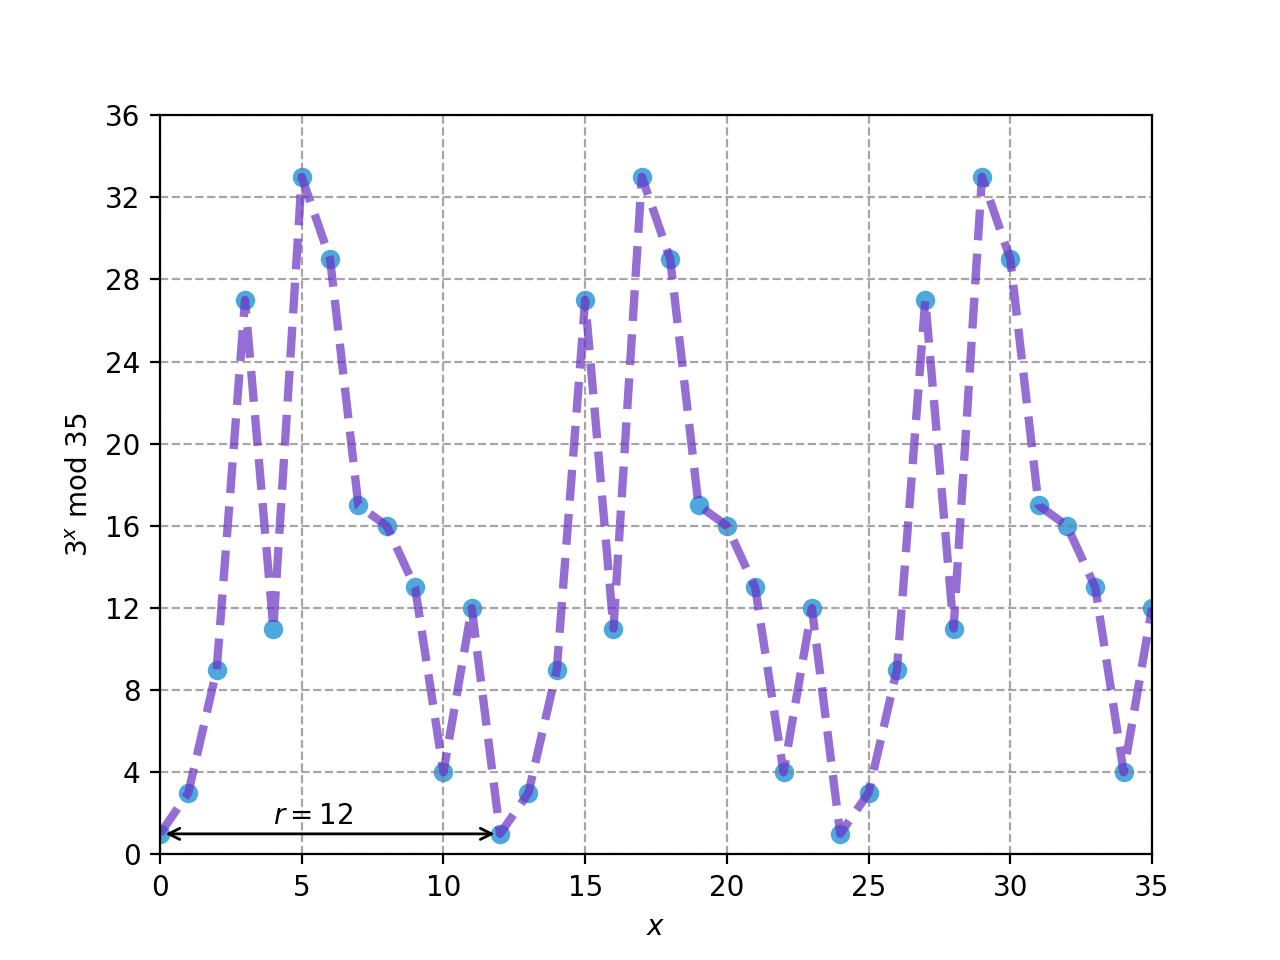
\includegraphics[scale=0.65]{../Graphics/period.png}
    \caption{Periodo de la función \ref{eq:axmodn} para visualizar la condición \ref{eq:condicionr} usando el código \ref{cod:rperiod}}
    \label{fig:condicionr}
\end{figure}
Para realizar esta operación dentro del Algoritmo de Shor se propusó un operador unitario tal que:
\begin{equation}
    U \left| y \right\rangle \equiv \left| ay mod N \right\rangle 
    \label{eq:umod}
\end{equation}
Para visualizar el funcionamiento de este operador se usará el ejemplo de $a=3$ y $N=35$, trabajando con los eigenestados de U empezando con el estado 
$\left|1\right\rangle$ podemos visualizar que la transformación sucesiva del operador U estariasmos multiplicando el estado por $amodN$, por lo tanto, después de
r transformaciones regresaremos al estado $\left|1\right\rangle$.
\begin{align*}
    U\left| 1 \right\rangle &= \left|3\right\rangle \\
    U^2\left| 1 \right\rangle &= \left|9\right\rangle \\
    U^3\left| 1 \right\rangle &= \left|12\right\rangle \\ 
                    & \vdots  \\ 
    U^{r-1}\left| 1 \right\rangle &= \left|12\right\rangle \\
    U^r\left| 1 \right\rangle &= \left|1\right\rangle \\
\end{align*}
Utilizando una superposición de estos estados, obtendremos lo siguiente:
\begin{equation}
    \left| u_0 \right\rangle = \frac{1}{\sqrt{r}} \sum\limits_{k=0}^{r-1} \left|a^k mod N \right\rangle.
    \label{eq:u0}
\end{equation}
Realizando esa serie para $a=3$ y $N=35$, encontramos que el estado descrito en \ref{eq:uo} es invariante bajo la transformación de U.
\begin{align*}
    \left| u_0 \right\rangle &= \frac{1}{\sqrt{12}} \left(\left|1\right\rangle + \left|3\right\rangle+ \left|9\right\rangle 
    +\cdots +\left|4\right\rangle + \left|12\right\rangle \right)\\
    U\left| u_0 \right\rangle &= \frac{1}{\sqrt{12}} \left(U\left|1\right\rangle + U\left|3\right\rangle+ U\left|9\right\rangle 
    +\cdots +U\left|4\right\rangle + U\left|12\right\rangle \right)\\
    &= \frac{1}{\sqrt{12}} \left(\left|3\right\rangle + \left|9\right\rangle+ \left|27\right\rangle 
    +\cdots +\left|12\right\rangle + \left|1\right\rangle \right)\\
    &= \left| u_0 \right\rangle .
\end{align*}
Lo cual obtenemos que el eigenvalor es 1. Un eigenestado más general es aquel el cual contenga una fase diferente para cada base de estados. Especificamente, veremos el caso
donde cada fase del k-esimo es proporcional a k, de tal manera que:
\begin{align}
    \label{eq:u1}
    \left| u_1 \right\rangle &= \frac{1}{\sqrt{r}} \sum\limits_{k=0}^{r-1} e^{-\frac{2\pi i k}{r}} \left| a^k mod N \right\rangle \\
    \label{eq:ua1}
    U\left| u_1 \right\rangle &= e^{\frac{2\pi i}{r}} \left| u_1 \right\rangle.
\end{align}
Teniendo así un único eigenestado para cada valor entero en $s$ donde $0\leq s \leq r-1$. Esto es muy conveniente, ya que realizando la suma de los eigenestados, las diferencias de fases
serán canceladas, obteniendo así el estado $ \left| 1 \right\rangle$.
\begin{equation*}
    \frac{1}{\sqrt{r}} \sum\limits_{s=0}^{r-1} \left|u_s \right\rangle =  \left| 1 \right\rangle.
\end{equation*}
Siendo así que el estado $ \left| 1 \right\rangle$ es una superposición de estos eigenestados, lo cual indica que podemos realizar 
QPE al opeeador U usando el estado $ \left| 1 \right\rangle$, para así obtener la medición de la fase:
\begin{equation*}
    \phi = \frac{s}{r}
\end{equation*}
Realizando del algoritmo de fracciones continuas sobre $\phi$ podemos encontrar el valor de ra. El circuito cuántico que realiza esta tarea es el siguiente:
\begin{figure}[H]
    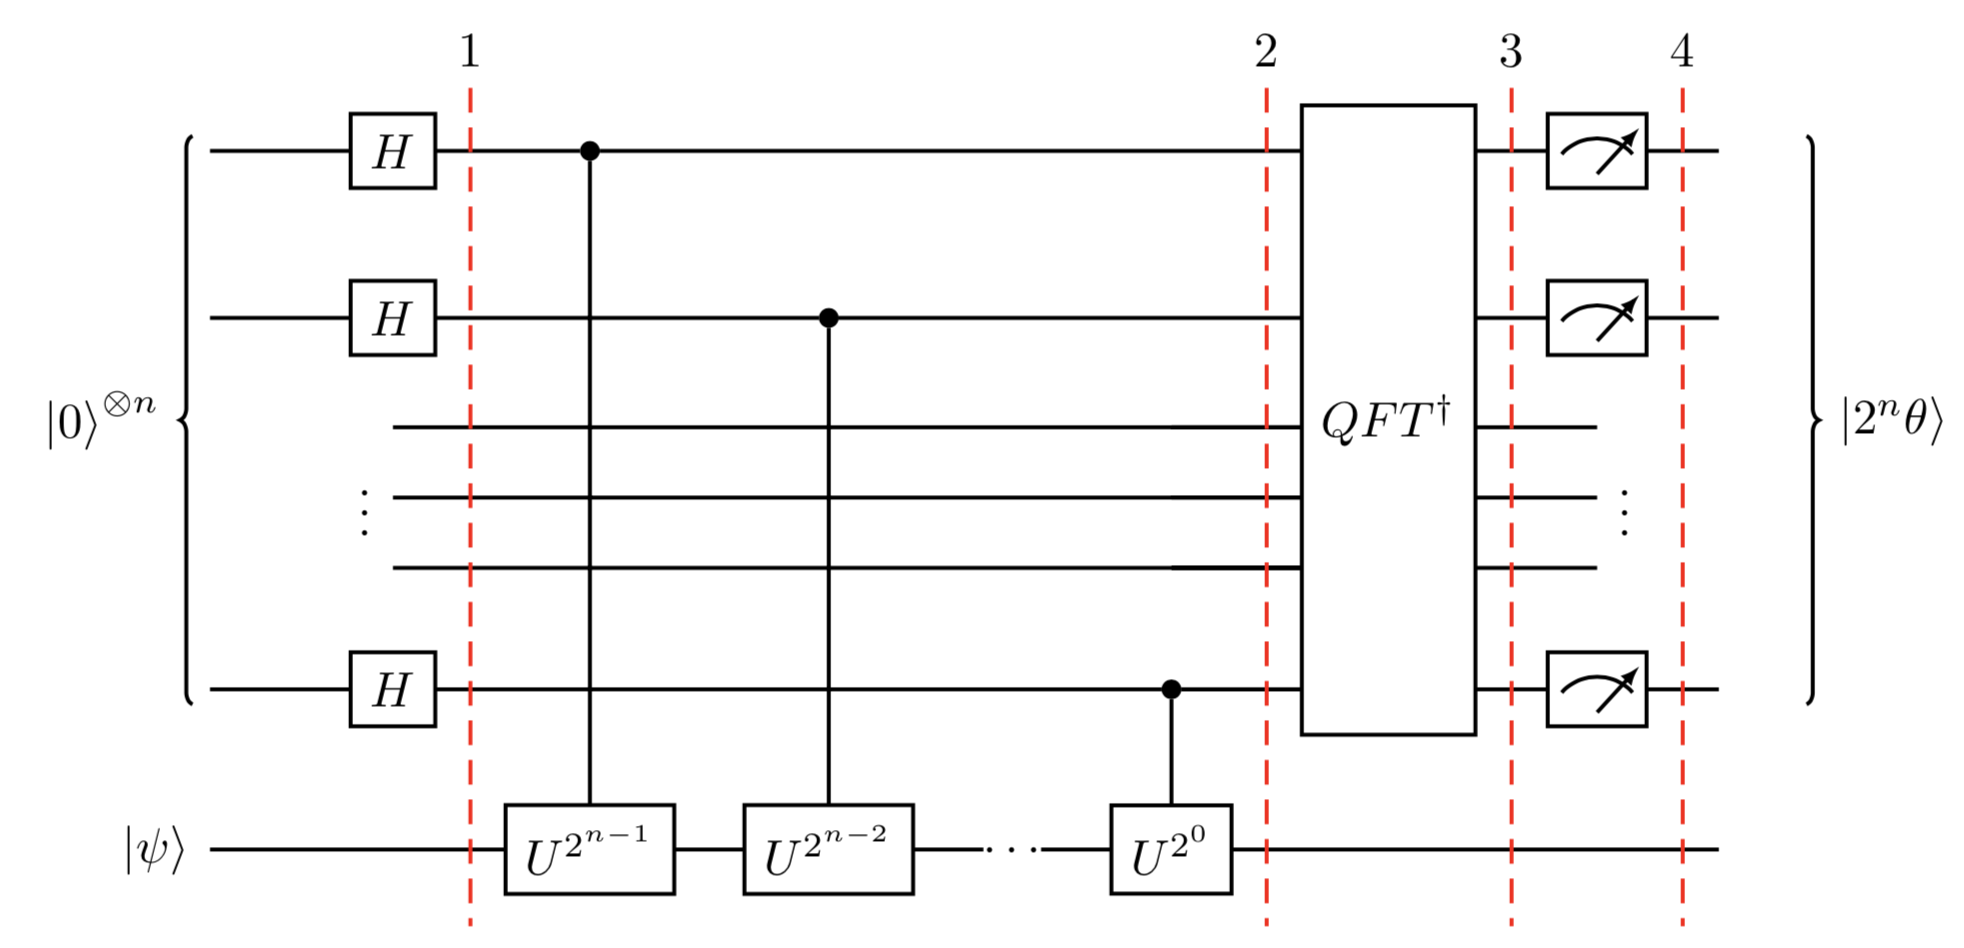
\includegraphics[scale=0.4]{../Graphics/qpe.png}
    \label{fig:qpe}
    \caption{Circuito cuántico que realiza el algortimo QPE sobre una serie de qubits.}
\end{figure}
\subsection{Implementación con Qiskit}
Para mostrar de forma detallada se trabajara con el problema cuando $a=7$ y $N=15$. Con esto, realizamos el operador U aplicado al estado $\left|y \right\rangle$ de la siguiente manera:
\begin{equation}
    U\left| y \right\rangle = \left|aymod15 \right\rangle 
    \label{eq:ua15}
\end{equation}
Para crear las operaciones acumulativas $U^x$, se creará una repetición del circuito $x$ veces, por lo que la función \textcolor{def}{\textit{c\_amod15}}
 regresará la compuerta U al valor de a y la añadira al circuito cuántico con la función \textcolor{def}{\textit{modular\_exponentiation}}, repetida x veces como lo siguiente:
 \begin{tcolorbox}[breakable, size=fbox, boxrule=1pt, pad at break*=1mm,colback=cellbackground, colframe=cellborder]
    \prompt{In}{incolor}{}{\boxspacing}
    \begin{Verbatim}[commandchars=\\\{\}]
    \PY{k}{def} \PY{n+nf}{c\PYZus{}amod15}\PY{p}{(}\PY{n}{a}\PY{p}{,} \PY{n}{x}\PY{p}{)}\PY{p}{:}
        \PY{k}{if} \PY{n}{a} \PY{o+ow}{not} \PY{o+ow}{in} \PY{p}{[}\PY{l+m+mi}{2}\PY{p}{,}\PY{l+m+mi}{7}\PY{p}{,}\PY{l+m+mi}{8}\PY{p}{,}\PY{l+m+mi}{11}\PY{p}{,}\PY{l+m+mi}{13}\PY{p}{]}\PY{p}{:}
            \PY{k}{raise} \PY{n+ne}{ValueError}\PY{p}{(}\PY{l+s+s2}{\PYZdq{}}\PY{l+s+s2}{\PYZsq{}}\PY{l+s+s2}{a}\PY{l+s+s2}{\PYZsq{}}\PY{l+s+s2}{ debe ser 2,7,8,11 o 13}\PY{l+s+s2}{\PYZdq{}}\PY{p}{)}
        \PY{n}{U} \PY{o}{=} \PY{n}{QuantumCircuit}\PY{p}{(}\PY{l+m+mi}{4}\PY{p}{)}        
        \PY{k}{for} \PY{n}{iteration} \PY{o+ow}{in} \PY{n+nb}{range}\PY{p}{(}\PY{n}{x}\PY{p}{)}\PY{p}{:}
            \PY{k}{if} \PY{n}{a} \PY{o+ow}{in} \PY{p}{[}\PY{l+m+mi}{2}\PY{p}{,}\PY{l+m+mi}{13}\PY{p}{]}\PY{p}{:}
                \PY{n}{U}\PY{o}{.}\PY{n}{swap}\PY{p}{(}\PY{l+m+mi}{0}\PY{p}{,}\PY{l+m+mi}{1}\PY{p}{)}
                \PY{n}{U}\PY{o}{.}\PY{n}{swap}\PY{p}{(}\PY{l+m+mi}{1}\PY{p}{,}\PY{l+m+mi}{2}\PY{p}{)}
                \PY{n}{U}\PY{o}{.}\PY{n}{swap}\PY{p}{(}\PY{l+m+mi}{2}\PY{p}{,}\PY{l+m+mi}{3}\PY{p}{)}
            \PY{k}{if} \PY{n}{a} \PY{o+ow}{in} \PY{p}{[}\PY{l+m+mi}{7}\PY{p}{,}\PY{l+m+mi}{8}\PY{p}{]}\PY{p}{:}
                \PY{n}{U}\PY{o}{.}\PY{n}{swap}\PY{p}{(}\PY{l+m+mi}{2}\PY{p}{,}\PY{l+m+mi}{3}\PY{p}{)}
                \PY{n}{U}\PY{o}{.}\PY{n}{swap}\PY{p}{(}\PY{l+m+mi}{1}\PY{p}{,}\PY{l+m+mi}{2}\PY{p}{)}
                \PY{n}{U}\PY{o}{.}\PY{n}{swap}\PY{p}{(}\PY{l+m+mi}{0}\PY{p}{,}\PY{l+m+mi}{1}\PY{p}{)}
            \PY{k}{if} \PY{n}{a} \PY{o}{==} \PY{l+m+mi}{11}\PY{p}{:}
                \PY{n}{U}\PY{o}{.}\PY{n}{swap}\PY{p}{(}\PY{l+m+mi}{1}\PY{p}{,}\PY{l+m+mi}{3}\PY{p}{)}
                \PY{n}{U}\PY{o}{.}\PY{n}{swap}\PY{p}{(}\PY{l+m+mi}{0}\PY{p}{,}\PY{l+m+mi}{2}\PY{p}{)}
            \PY{k}{if} \PY{n}{a} \PY{o+ow}{in} \PY{p}{[}\PY{l+m+mi}{7}\PY{p}{,}\PY{l+m+mi}{11}\PY{p}{,}\PY{l+m+mi}{13}\PY{p}{]}\PY{p}{:}
                \PY{k}{for} \PY{n}{q} \PY{o+ow}{in} \PY{n+nb}{range}\PY{p}{(}\PY{l+m+mi}{4}\PY{p}{)}\PY{p}{:}
                    \PY{n}{U}\PY{o}{.}\PY{n}{x}\PY{p}{(}\PY{n}{q}\PY{p}{)}
        \PY{n}{U} \PY{o}{=} \PY{n}{U}\PY{o}{.}\PY{n}{to\PYZus{}gate}\PY{p}{(}\PY{p}{)}
        \PY{n}{U}\PY{o}{.}\PY{n}{name} \PY{o}{=} \PY{l+s+s2}{\PYZdq{}}\PY{l+s+si}{\PYZpc{}i}\PY{l+s+s2}{\PYZca{}}\PY{l+s+si}{\PYZpc{}i}\PY{l+s+s2}{ mod 15}\PY{l+s+s2}{\PYZdq{}} \PY{o}{\PYZpc{}} \PY{p}{(}\PY{n}{a}\PY{p}{,} \PY{n}{x}\PY{p}{)}
        \PY{n}{c\PYZus{}U} \PY{o}{=} \PY{n}{U}\PY{o}{.}\PY{n}{control}\PY{p}{(}\PY{p}{)}
        \PY{k}{return} \PY{n}{c\PYZus{}U}
    \PY{k}{def} \PY{n+nf}{modular\PYZus{}exponentiation}\PY{p}{(}\PY{n}{given\PYZus{}circuit}\PY{p}{,} \PY{n}{n}\PY{p}{,} \PY{n}{m}\PY{p}{,} \PY{n}{a}\PY{p}{)}\PY{p}{:}
        \PY{k}{for} \PY{n}{x} \PY{o+ow}{in} \PY{n+nb}{range}\PY{p}{(}\PY{n}{n}\PY{p}{)}\PY{p}{:}
            \PY{n}{exponent} \PY{o}{=} \PY{l+m+mi}{2}\PY{o}{*}\PY{o}{*}\PY{n}{x}
            \PY{n}{given\PYZus{}circuit}\PY{o}{.}\PY{n}{append}\PY{p}{(}\PY{n}{a\PYZus{}x\PYZus{}mod15}\PY{p}{(}\PY{n}{a}\PY{p}{,} \PY{n}{exponent}\PY{p}{)}\PY{p}{,} 
                         \PY{p}{[}\PY{n}{x}\PY{p}{]} \PY{o}{+} \PY{n+nb}{list}\PY{p}{(}\PY{n+nb}{range}\PY{p}{(}\PY{n}{n}\PY{p}{,} \PY{n}{n}\PY{o}{+}\PY{n}{m}\PY{p}{)}\PY{p}{)}\PY{p}{)}
    \end{Verbatim}
    \end{tcolorbox}
Al algortimo también se le implemento la transformación inversa de Fourier cuántica, se le nombre como \textcolor{def}{\textit{qft\_dagger}}, esta función es la siguiente:
\begin{tcolorbox}[breakable, size=fbox, boxrule=1pt, pad at break*=1mm,colback=cellbackground, colframe=cellborder]
    \prompt{In}{incolor}{}{\boxspacing}
    \begin{Verbatim}[commandchars=\\\{\}]
    \PY{k}{def} \PY{n+nf}{qft\PYZus{}dagger}\PY{p}{(}\PY{n}{n}\PY{p}{)}\PY{p}{:}
        \PY{n}{qc} \PY{o}{=} \PY{n}{QuantumCircuit}\PY{p}{(}\PY{n}{n}\PY{p}{)}
        \PY{k}{for} \PY{n}{qubit} \PY{o+ow}{in} \PY{n+nb}{range}\PY{p}{(}\PY{n}{n}\PY{o}{/}\PY{o}{/}\PY{l+m+mi}{2}\PY{p}{)}\PY{p}{:}
            \PY{n}{qc}\PY{o}{.}\PY{n}{swap}\PY{p}{(}\PY{n}{qubit}\PY{p}{,} \PY{n}{n}\PY{o}{\PYZhy{}}\PY{n}{qubit}\PY{o}{\PYZhy{}}\PY{l+m+mi}{1}\PY{p}{)}
        \PY{k}{for} \PY{n}{j} \PY{o+ow}{in} \PY{n+nb}{range}\PY{p}{(}\PY{n}{n}\PY{p}{)}\PY{p}{:}
            \PY{k}{for} \PY{n}{m} \PY{o+ow}{in} \PY{n+nb}{range}\PY{p}{(}\PY{n}{j}\PY{p}{)}\PY{p}{:}
                \PY{n}{qc}\PY{o}{.}\PY{n}{cu1}\PY{p}{(}\PY{o}{\PYZhy{}}\PY{n}{np}\PY{o}{.}\PY{n}{pi}\PY{o}{/}\PY{n+nb}{float}\PY{p}{(}\PY{l+m+mi}{2}\PY{o}{*}\PY{o}{*}\PY{p}{(}\PY{n}{j}\PY{o}{\PYZhy{}}\PY{n}{m}\PY{p}{)}\PY{p}{)}\PY{p}{,} \PY{n}{m}\PY{p}{,} \PY{n}{j}\PY{p}{)}
            \PY{n}{qc}\PY{o}{.}\PY{n}{h}\PY{p}{(}\PY{n}{j}\PY{p}{)}
        \PY{n}{qc}\PY{o}{.}\PY{n}{name} \PY{o}{=} \PY{l+s+s2}{\PYZdq{}}\PY{l+s+s2}{iqft}\PY{l+s+s2}{\PYZdq{}}
        \PY{k}{return} \PY{n}{qc}
    \end{Verbatim}
    \end{tcolorbox}
Ya con estas funciones preestablecidas, el algoritmo de Shor es construido de una manera amigable a la vista, este es el siguiente:
\begin{tcolorbox}[breakable, size=fbox, boxrule=1pt, pad at break*=1mm,colback=cellbackground, colframe=cellborder]
    \prompt{In}{incolor}{}{\boxspacing}
    \begin{Verbatim}[commandchars=\\\{\}]
    \PY{k}{def} \PY{n+nf}{shor\PYZus{}program}\PY{p}{(}\PY{n}{n}\PY{p}{,} \PY{n}{m}\PY{p}{,} \PY{n}{a}\PY{p}{)}\PY{p}{:}
        \PY{c+c1}{\PYZsh{} set up quantum circuit}
        \PY{n}{shor} \PY{o}{=} \PY{n}{QuantumCircuit}\PY{p}{(}\PY{n}{n}\PY{o}{+}\PY{n}{m}\PY{p}{,} \PY{n}{n}\PY{p}{)}
        \PY{c+c1}{\PYZsh{} initialize the qubits}
        \PY{n}{initialize\PYZus{}qubits}\PY{p}{(}\PY{n}{shor}\PY{p}{,} \PY{n}{n}\PY{p}{,} \PY{n}{m}\PY{p}{)}
        \PY{n}{shor}\PY{o}{.}\PY{n}{barrier}\PY{p}{(}\PY{p}{)}
        \PY{c+c1}{\PYZsh{} apply modular exponentiation}
        \PY{n}{modular\PYZus{}exponentiation}\PY{p}{(}\PY{n}{shor}\PY{p}{,} \PY{n}{n}\PY{p}{,} \PY{n}{m}\PY{p}{,} \PY{n}{a}\PY{p}{)}
        \PY{n}{shor}\PY{o}{.}\PY{n}{barrier}\PY{p}{(}\PY{p}{)}
        \PY{c+c1}{\PYZsh{} apply inverse QFT}
        \PY{n}{apply\PYZus{}iqft}\PY{p}{(}\PY{n}{shor}\PY{p}{,} \PY{n+nb}{range}\PY{p}{(}\PY{n}{n}\PY{p}{)}\PY{p}{)}
        \PY{c+c1}{\PYZsh{} measure the first n qubits}
        \PY{n}{shor}\PY{o}{.}\PY{n}{measure}\PY{p}{(}\PY{n+nb}{range}\PY{p}{(}\PY{n}{n}\PY{p}{)}\PY{p}{,} \PY{n+nb}{range}\PY{p}{(}\PY{n}{n}\PY{p}{)}\PY{p}{)}
        \PY{k}{return} \PY{n}{shor}
    \PY{n}{n} \PY{o}{=} \PY{l+m+mi}{4}\PY{p}{;} \PY{n}{m} \PY{o}{=} \PY{l+m+mi}{4}\PY{p}{;} \PY{n}{a} \PY{o}{=} \PY{l+m+mi}{7}
    \PY{n}{mycircuit} \PY{o}{=} \PY{n}{shor\PYZus{}program}\PY{p}{(}\PY{n}{n}\PY{p}{,} \PY{n}{m}\PY{p}{,} \PY{n}{a}\PY{p}{)}
    \PY{n}{mycircuit}\PY{o}{.}\PY{n}{draw}\PY{p}{(}\PY{n}{output}\PY{o}{=}\PY{l+s+s1}{\PYZsq{}}\PY{l+s+s1}{text}\PY{l+s+s1}{\PYZsq{}}\PY{p}{)}
    \end{Verbatim}
    \end{tcolorbox}
Al termino de estas lineas de código tendremos la serie de posibles factores primos del número 15, por lo que con ayuda de un algoritmo clásico se podra comprobar si los cálculos 
antes realizados son correctos, este algoritmo es el siguiente:
\begin{tcolorbox}[breakable, size=fbox, boxrule=1pt, pad at break*=1mm,colback=cellbackground, colframe=cellborder]
    \prompt{In}{incolor}{}{\boxspacing}
    \begin{Verbatim}[commandchars=\\\{\}]
    \PY{k+kn}{from} \PY{n+nn}{math} \PY{k}{import} \PY{n}{gcd}
    
    \PY{k}{for} \PY{n}{measured\PYZus{}value} \PY{o+ow}{in} \PY{n}{counts}\PY{p}{:}
        \PY{n}{measured\PYZus{}value\PYZus{}decimal} \PY{o}{=} \PY{n+nb}{int}\PY{p}{(}\PY{n}{measured\PYZus{}value}\PY{p}{[}\PY{p}{:}\PY{p}{:}\PY{o}{\PYZhy{}}\PY{l+m+mi}{1}\PY{p}{]}\PY{p}{,} \PY{l+m+mi}{2}\PY{p}{)}
        \PY{n+nb}{print}\PY{p}{(}\PY{n}{f}\PY{l+s+s2}{\PYZdq{}}\PY{l+s+s2}{Medición }\PY{l+s+si}{\PYZob{}measured\PYZus{}value\PYZus{}decimal\PYZcb{}}\PY{l+s+s2}{\PYZdq{}}\PY{p}{)}
        
        \PY{k}{if} \PY{n}{measured\PYZus{}value\PYZus{}decimal} \PY{o}{\PYZpc{}} \PY{l+m+mi}{2} \PY{o}{!=} \PY{l+m+mi}{0}\PY{p}{:}
            \PY{n+nb}{print}\PY{p}{(}\PY{l+s+s2}{\PYZdq{}}\PY{l+s+s2}{Fallo. El número no es par}\PY{l+s+s2}{\PYZdq{}}\PY{p}{)}
            \PY{k}{continue}
        \PY{n}{x} \PY{o}{=} \PY{n+nb}{int}\PY{p}{(}\PY{p}{(}\PY{n}{a} \PY{o}{*}\PY{o}{*} \PY{p}{(}\PY{n}{measured\PYZus{}value\PYZus{}decimal}\PY{o}{/}\PY{l+m+mi}{2}\PY{p}{)}\PY{p}{)} \PY{o}{\PYZpc{}} \PY{l+m+mi}{15}\PY{p}{)}
        \PY{k}{if} \PY{p}{(}\PY{n}{x} \PY{o}{+} \PY{l+m+mi}{1}\PY{p}{)} \PY{o}{\PYZpc{}} \PY{l+m+mi}{15} \PY{o}{==} \PY{l+m+mi}{0}\PY{p}{:}
            \PY{n+nb}{print}\PY{p}{(}\PY{l+s+s2}{\PYZdq{}}\PY{l+s+s2}{Fallo. x + 1 = 0 (mod N) donde x = a\PYZca{}(r/2) (mod N)}\PY{l+s+s2}{\PYZdq{}}\PY{p}{)}
            \PY{k}{continue}
        \PY{n}{guesses} \PY{o}{=} \PY{n}{gcd}\PY{p}{(}\PY{n}{x} \PY{o}{+} \PY{l+m+mi}{1}\PY{p}{,} \PY{l+m+mi}{15}\PY{p}{)}\PY{p}{,} \PY{n}{gcd}\PY{p}{(}\PY{n}{x} \PY{o}{\PYZhy{}} \PY{l+m+mi}{1}\PY{p}{,} \PY{l+m+mi}{15}\PY{p}{)}
        \PY{n+nb}{print}\PY{p}{(}\PY{n}{guesses}\PY{p}{)}
    \end{Verbatim}
    \end{tcolorbox}
Dando como resultado lo siguiente:
        \begin{Verbatim}[commandchars=\\\{\}]
    Medición 0
    (1, 15)
    Medición 8
    (1, 15)
    Medición 4
    (5, 3)
    Medición 12
    (5, 3)
        \end{Verbatim}
En donde se puede observar que no necesariamente el algoritmo cuántico encontrará la factorización que nosotros esperariamos, si no que necesita ayuda de una computadora clásica para comprobar sus resultados. Este circuito esta hecho Especificamente
para factorizar el número 15, el circuito cuántico que factoriza cualquier número N es el siguiente:
\begin{figure}[H]
    \centering
    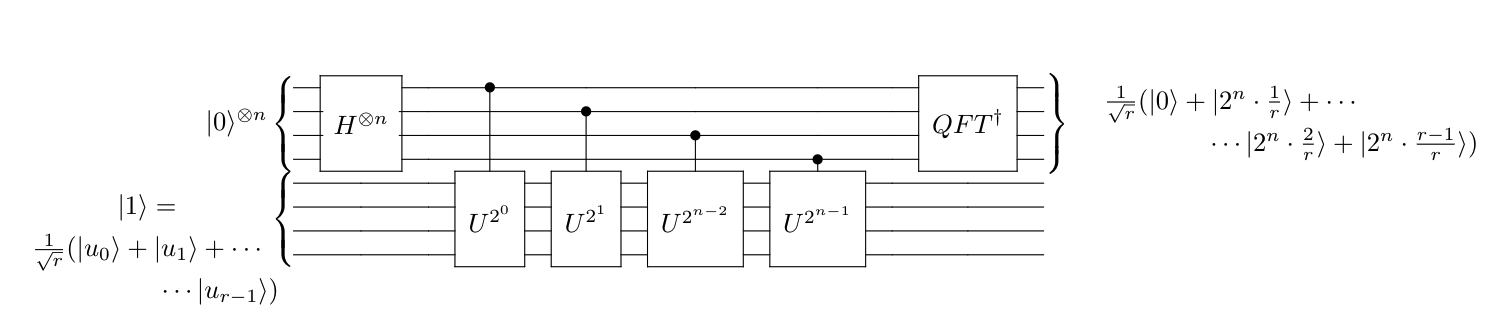
\includegraphics[scale=0.3]{../Graphics/shor_circuit.png}
    \caption{Algoritmo de Shor para la factorización de un número visto desde la estructura que propone Qiskit.}
    \label{fig:shorcircuit}
\end{figure}